\documentclass[a4paper, 11pt]{article}

\usepackage[french]{babel}
\usepackage[T1]{fontenc}
\usepackage[utf8]{inputenc}
\usepackage{hyperref}
\usepackage{graphicx}
\usepackage{xcolor}
\usepackage{fullpage}

\usepackage{fancyvrb}

\usepackage{amsmath}
\usepackage{amsthm}
\usepackage{amssymb}
\usepackage{comment}

\hypersetup{
    colorlinks,
    linkcolor={black!50!black},
    citecolor={black!50!black},
    urlcolor={black!80!black}
}

\VerbatimFootnotes

\newcommand\todo[1]{\textcolor{red}{TODO: #1}\PackageWarning{TODO:}{#1!}}
\newcommand\Order{\mathop{\operator@font O}\nolimits}% big O of ...

\newtheorem*{exemple}{Exemple}


\begin{document}

\begin{titlepage}
\begin{center}

{\Large Université de Mons}\\[1ex]
{\Large Faculté des sciences}\\[2.5cm]

\newcommand{\HRule}{\rule{\linewidth}{0.3mm}}
% Title
\HRule \\[0.3cm]
{ \LARGE \bfseries Assemblage de fragments d'ADN \\[0.3cm]}
\HRule \\[1.5cm]

% Course
\begin{center}
\emph{Cours:} \\
Algorithmique et bioinformatique
\end{center}

% Author
\begin{center}
\emph{Auteurs:} \\
Aline \textsc{Goeminne}\\
Danny \textsc{Willems}
\end{center}
\vfill
\today
\vfill

% Bottom of the page
\begin{center}
\begin{tabular}[t]{c c c}

\includegraphics[height=1.5cm]{umons.jpg} &
\hspace{0.3cm} &

\includegraphics[height=1.5cm]{fac.jpg}
\end{tabular}
\end{center}~\\

{\large Année académique 2015-2016}

\end{center}
\end{titlepage}

\tableofcontents
\newpage

%!TEX root=rapport.tex

\section{Introduction}

En biologie, il arrive qu'à partir d'un ensemble de fragments d'ADN on désire retrouver la séquence initiale correspondant à ces fragments.
C'est la tâche qui nous a été demandée. 

Le principe ne se résume pas simplement à prendre chaque fragment et à les mettre bout à bout afin de construire une super-chaîne. En effet,
comme les fragments ne sont pas coupés \og bout à bout\fg~ils se recouvrent partiellement. De plus, il se peut que lors de la fragmentation de l'ADN des nucléotides se soient rajoutés ou au contraire aient disparu (indel). De plus, si les deux brins d'ADN ont été fragmentés en même temps, il faut tenir compte du fait qu'un des brins est dans le sens \textbf{5'-3'} tandis que l'autre est dans le sens \textbf{3'-5'} et correspond au complémentaire du premier.

Notre rapport est rédigé de la manière suivante: dans la section suivante nous expliquons comment nous avons implémenté une solution à ce problème. Nous commençons par en expliquer brièvement chaque étape et ensuite nous expliquons plus précisément chacune d'elles. Ensuite, nous exposons et interprétons les résultats obtenus. Enfin, nous explicitons les forces et faiblesses que, d'après nous, notre implémentation comporte.

%!TEX root=rapport.tex
\section{Implémentation}

\subsection{Idée générale}

	L'idée générale de l'alignement de séquences est de permettre à partir d'un ensemble de séquences de créer à l'aide de chevauchements approximatif un \emph{contig}. Pour se faire, notre démarche se découpe en plusieurs parties:
	
	\begin{description}
		\item[Récupération et stockage des données] Afin de pouvoir former le contig souhaité, il est nécessaire de récupérer les séquences et de les stocker de manière efficaces. Cette étape est expliquée dans la section~\ref{subsection:recStock}.
		
		\item[Alignement semi-global] Ensuite, pour chaque paire de séquence, nous effectuons un \emph{alignement semi-global} en nous inspirant de l'algorithme vu en cours.Cette méthode nous donne ainsi l'alignement approximatif des deux séquences. Ce qui permet de prendre en compte le fait qu'il ait pu y avoir des erreurs lors du séquençage. Cette étape est expliquée dans la section~\ref{subsection:semiGlobal}.
		
		\item[Algorithme greedy] Une fois les alignements approximatifs calculés, il est encore nécessaire de trouver dans quel ordre ceux-ci doivent être assemblés afin de former le meilleur contig. Pour se faire, nous utilisons un \emph{algorithme greedy} qui, à partir d'un graphe permet de trouver un chemin hamiltonien afin de reconstituer le contig. Cette étape est expliquée dans la section~\ref{subsection:greedy}.
		
		\item[Alignement]
		
		\item[Consensus]
		
	\end{description}

\subsection{Récupération et stockage des données}
\label{subsection:recStock}

Cette étape est effectuée au travers des classes \verb|FastaReader| et \verb|Alignement|. De plus, la classe \verb|FastaWriter| est utilisée afin de récupérer le résultat du procédé visant à trouver le meilleur contig.\\

La classe \verb|Alignment| permet de stocker sous forme d'un table de Bytes un fragment d'ADN. Nous prenons la convention suivante quant à la représentation des nucléotides et d'un gap:
	\begin{center}
		\begin{tabular}{|l|c|}
			\hline
			Nucléotide/Gap & Représentation \\
			\hline
			\hline
			C & int 0 \\
			\hline
			G & int 1\\
			\hline
			T & int 2 \\
			\hline
			A & int 3 \\
			\hline
			Gap & int 4 \\
			\hline

		\end{tabular}
	\end{center}
	
	Le fait de stocker les nucléotides sous forme de Bytes permet de réduire l'espace mémoire nécessaire.
		
	  Elle contient également des méthodes intéressantes telles que \textsc{complement} qui permet de complémenter une séquence d'ADN ainsi que d'autres méthodes comme \textsc{backTrack} et \textsc{semiGlobalAlignment} qui sont utiles pour l'étape décrire dans la section~\ref{subsection:semiGlobal} ou encore \textsc{arcGenerator} qui est expliquée dans la section~\ref{subsection:greedy}.\\
	
La classe \verb|FastaReader| permet à partir d'un \emph{fichier Fasta} de générer un liste d'objets \verb|Sequence| représentant les fragments d'ADN. \\

L'opération inverse est possible grâce à la classe \verb|FastaWriter|.


	


\subsection{Alignement semi-global}
\label{subsection:semiGlobal}

Une des premières étapes de la démarche est d'effectuer l'alignement semi-global entre deux fragments. Cette étape permet de tester la similarité entre les deux fragments que l'on veut aligner. L'alignement semi-global est implémenté dans la classe \verb|Sequence| via la fonction \textsc{semiGlobalAlignement}. Cette méthode prend deux fragments $s$ et $t$, des coûts de match, missmatch et gap  et calcule l'alignement de $s$ par rapport à $t$ et $t$ par rapport à $s$ et revoie le résultat sous forme d'une liste de \verb|SequenceAlignement|.\\

Un objet de la classe \verb|SequenceAlignement| est défini de la manière suivante: le segment $s_1$ aligné avec le segment $s_2$ en supposant que le segment $s_1$ est le segment le plus à \og gauche \fg. De plus, la longueur du préfix-suffix commun est stocké dans l'attribut \emph{score}.\\

De plus, dans la classe \verb|Sequence| nous retrouvons la méthode \emph{arcGenerator} qui à partir de deux fragments $s_1$ et $s_2$ calcule tous les alignements possibles. C'est-à-dire, si on considère que $\overline{s_1}$ est le fragment complémentaire inversé de $s_1$, alors on calcule:\\
\begin{itemize}
	\item[$\bullet$] L'alignement $(s_1,s_2)$ ainsi que $(s_2,s_1)$;
	\item[$\bullet$] L'alignement de $(\overline{s_1},s_2)$ ainsi que $(s_2, \overline{s_1})$;
	\item[$\bullet$] L'alignement de $(s_1, \overline{s_2})$ ainsi que $(\overline{s_2},s_1)$;
	\item[$\bullet$] L'alignement de $(\overline{s_1}, \overline{s_2})$ ainsi que $(\overline{s_2}, \overline{s_1})$.
\end{itemize}
$ $\\
A partir de ces alignements nous construisons les objets \verb|Arc|. Un objet arc possède en attribut:\\

\begin{itemize}
	\item[$\bullet$] Les fragments $s_1$ et $s_2$ initiaux qui sont utilisés lors de l'alignement.
	\item[$\bullet$] Des booléens \emph{s1Comp} et \emph{s1Comp} qui permettent de savoir si on considère le complémentaire inversé lors de l'alignement.
	\item[$\bullet$] Les alignements \emph{s1Aligned} et \emph{s2Aligned}  résultant de l'exécution de l'algorithme d'alignement semi-global.
\end{itemize}
	
Ces arcs nous permettent d'effectuer l'algorithme greedy pour trouver un chemin hamiltonien parcourant tous les fragments considérés.


\subsection{Algorithme greedy}
\label{subsection:greedy}

Avant de nous intéresser à l'algorithme greedy en tant que tel, nous allons expliquer une structure de données \emph{Union-Find} que nous avons utilisée afin d'implémenter cet algorithme.

\subsubsection{Union-Find}

Une structure de donnée \og Union-Find \fg~est une structure permettant de représenter une relation d'équivalence . On peut effectuer trois opérations sur cette structure:
\begin{itemize}
\item[$\bullet$] L'opération \textsc{Find} permet de déterminer dans quelle classe d'équivalence se situe un élément.
\item[$\bullet$] L'opération \textsc{Union} permet de faire l'union entre deux classes d'équivalence.
\item[$\bullet$] L'opération \textsc{MakeSet} construit une classe d'équivalence qui ne contient qu'un seul élément
\end{itemize}

Dans l'implémentation que nous avons utilisée, chaque classe d'équivalence est représentée par un arbre pour lequel chaque noeud possède une référence vers son père. Dans un tel choix d'implémentation, la racine de chaque classe correspond au représentant de la classe d'équivalence.

L'idée est que l'opération \textsc{Find} permet de retourner à la racine de l'arbre et donc de déterminer quel est le représentant de la classe d'équivalence. Pour l'opération \textsc{Union}, on rattache la racine d'une des deux classes à celle de l'autre classe. Toutefois, une telle démarche pourrait amener à des arbres fortement déséquilibrés . Afin d'éviter cela, une heuristique sur la hauteur de l'arbre est utilisée. On retient le \emph{rang} de l'arbre et à chaque fois que l'on veut faire l'union de deux arbres on considère leur rang. On attache l'arbre de rang inférieur à la racine de l'arbre de rang supérieur. Les arbres qui ne contiennent qu'un seul élément sont de rang 0 et dès que l'on effectue l'union de deux arbres de même rang, le résultat de cette union a un rang d'une unité plus grand.
%!TEX root=rapport.tex

\section{Interprétation des résultats obtenus}

\subsection{Résultats finaux}

Pour étudier les résultats que notre programme nous retourne, nous avons utilisé
un \textit{dotmatcher}.
Le principe du dotmatcher est de comparer deux séquences $s$ et $t$ données en
entrée: le dotmatcher parcourt les séquences en comparant chaque nucléotide
entre eux.  Lorsqu'une correspondance est faite, un point est tracé sur un
graphique. Une option, appelée \textit{thresold} peut être ajustée pour dissiper
le bruit. Une valeur de 50, suggérée lors du cours, a été utilisée pour cette
option.

Pour chaque nucléotide $s_{i}$ de la séquence $s$ et chaque nucléotide $t_{j}$
de la séquence $t$, le dotmatcher va tracer un point s'il y a une correspondance
entre les deux nucléotides.

Pour chaque comparaison de séquences, nous obtenons donc un rectangle de
points. Sur l'axe X, nous avons la longueur de la séquence que nous devons
obtenir, et sur l'axe Y, nous avons la longueur de la séquence que nous avons
obtenue.

Nous souhaitons, à travers ces graphiques, étudier la qualité de notre
résultat en regardant si chaque morceau de la séquence cible est bien
atteinte. Ceci se remarque par la présence de segments de droites car ceux-ci
reflètent une suite de nucléotides qui correspondent. Pour cela, il
suffit de projeter chaque segment obtenu sur l'axe X et regarder si l'ensemble
recouvre globalement la séquence de départ.

\subsubsection*{Cible 1}

Au niveau de la première cible (voir figure~\ref{cible1}), nous remarquons d'abord que la séquence que nous
avons obtenue est plus longue que la séquence cible fournie ($\simeq$ 14 000 vs
$\simeq$ 9000).

Les résultats sont meilleurs pour le normal que pour son complémentaire
inversé. Le recouvrement du premier est presque global, les intervalles non
couverts se trouvant aux alentours de 1000 et 7000. Quant au complémentaire
inversé, il y a un intervalle non couvert entre 2000 et 4000 ainsi que des
petits intervalles entre chaque segment.

Nous remarquons, à travers les droites, que nous avons de longues successions de
correspondances.

\begin{figure}[!ht]
	\begin{minipage}[r]{.46\linewidth}
		\begin{center}
		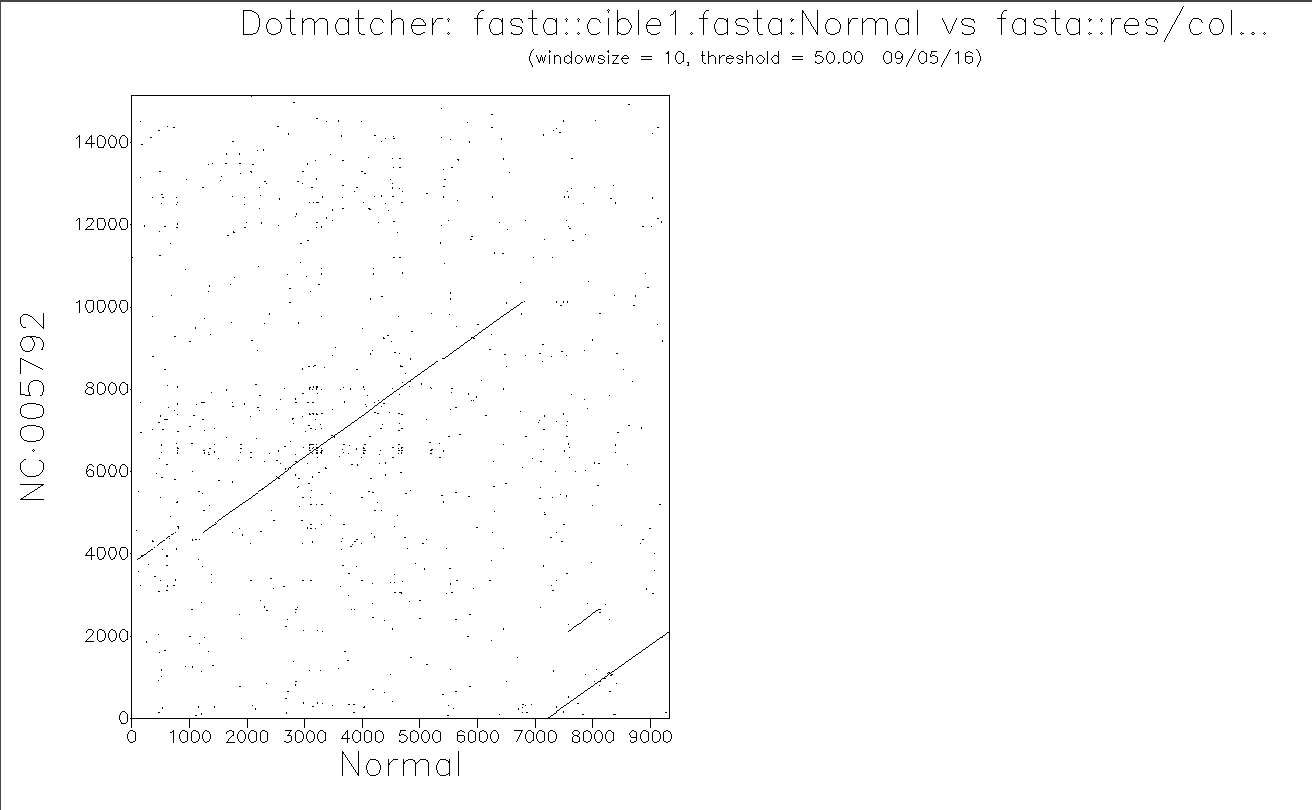
\includegraphics[scale= 0.7]{../res/cible1.png}
		Sequence obtenue
			\end{center}
\end{minipage} \hfill
\begin{minipage}[c]{.46 \linewidth}
	\begin{center}
			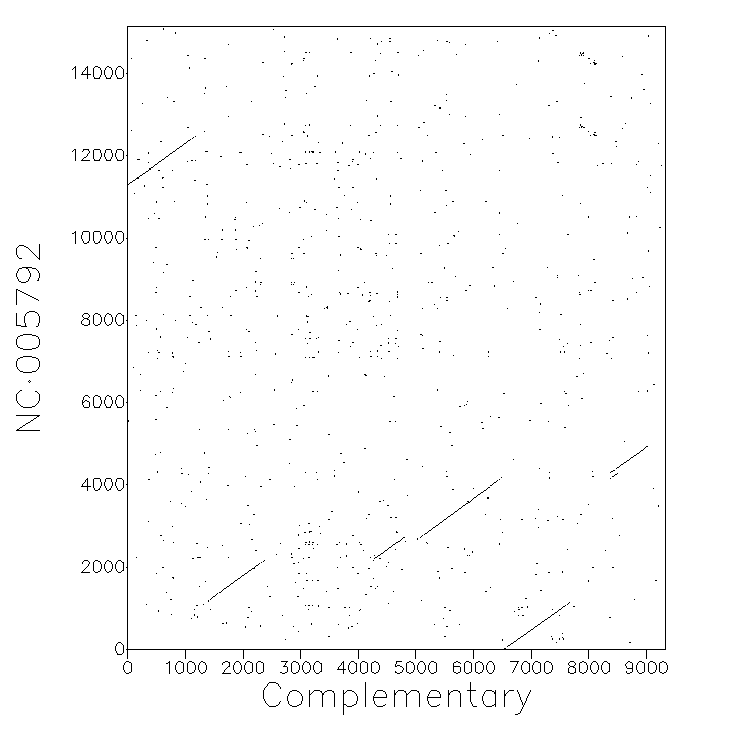
\includegraphics[scale= 0.7]{../res/cible1-ic.png}
			 Séquence complémentée et inversée
		\end{center}
	\end{minipage}
	\caption{Résultat de la collection 1}
	\label{cible1}
\end{figure}

\FloatBarrier

\subsubsection*{Cible 2}

Quant à la seconde cible (voir figure~\ref{cible2}), nous pouvons remarquer qu'il y a peu de
correspondances. Cependant, si nous zoomons sur certaines zones, nous pouvons
voir apparaitre des petits segments de droites.

Nous obtenons également une plus grande séquence: la cible contient environ
118000 nucléotides tandis que notre alignement en contient 190000.

\begin{figure}[!ht]
	\begin{minipage}[r]{.46\linewidth}
		\begin{center}
		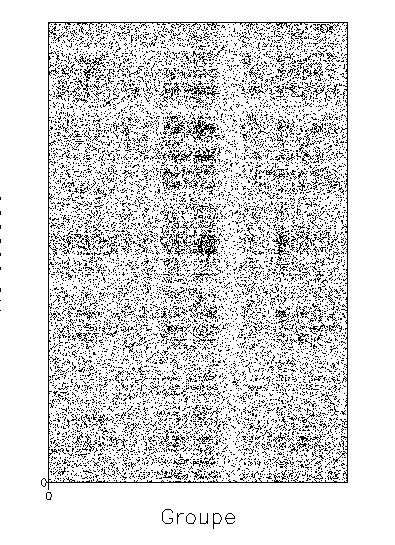
\includegraphics[scale=0.7]{../res/cible2.png}
Séquence obtenue	\end{center}
\end{minipage} \hfill
\begin{minipage}[c]{.46 \linewidth}
	\begin{center}
			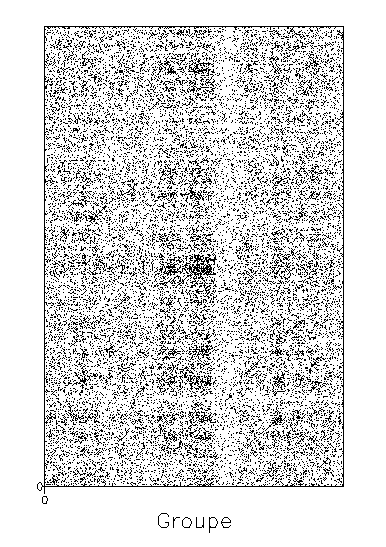
\includegraphics[scale=0.7]{../res/cible2-ic.png}
			 Séquence complémentée et inversée
		\end{center}
	\end{minipage}
	\caption{Résultat de la collection 2}
	\label{cible2}
\end{figure}

\FloatBarrier

\subsubsection*{Cible 4}

Les résultats pour la cible 4 (voir figure~\ref{cible4}) sont plutôt satisfaisants comme pour les cibles 1
et 5. Nous obtenons un recouvrement quasi-global ainsi qu'une longue droite
recouvrant à elle seule environ 65\% de la séquence cible.

Pour son complémentaire inversé, le recouvrement est plus éparpillé mais reste
tout de même assez global.

Comme les 2 premières séquences, nous obtenons une séquence plus longue.

\begin{figure}[!ht]
	\begin{minipage}[r]{.46\linewidth}
		\begin{center}
		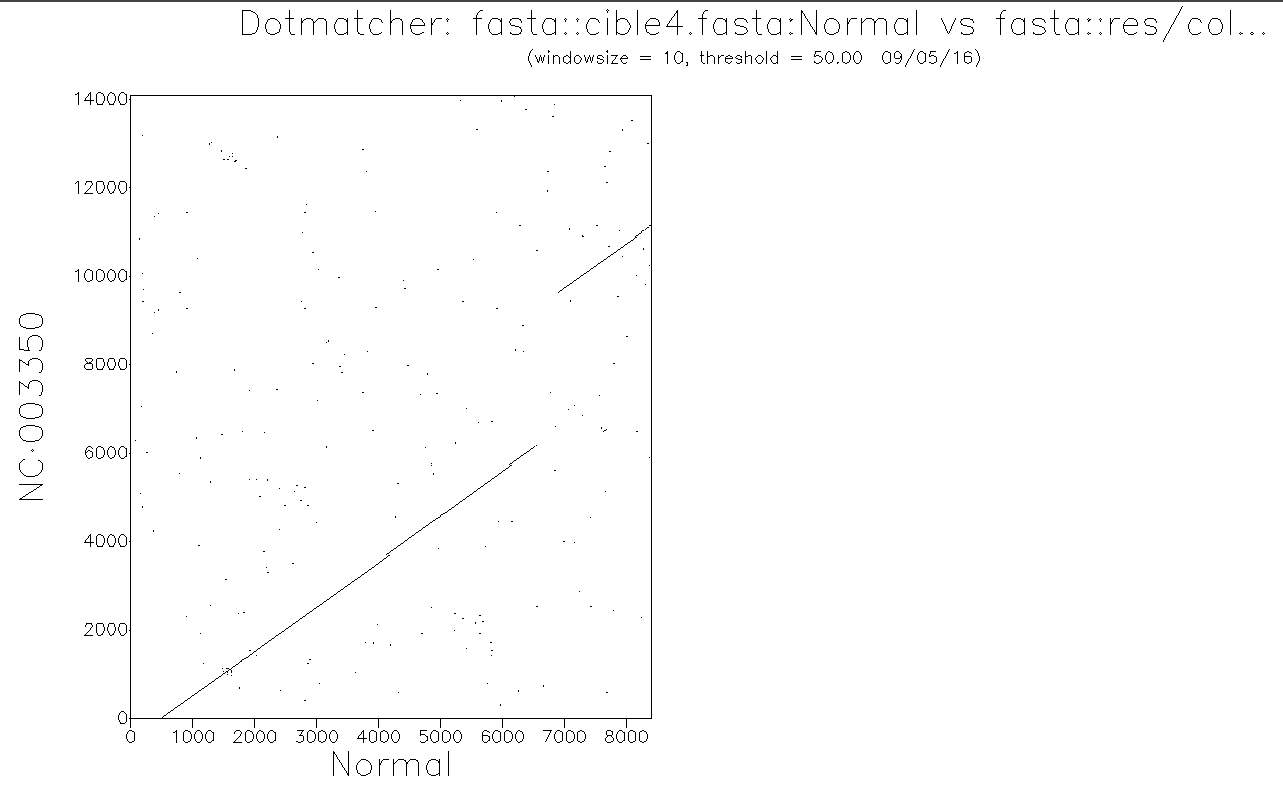
\includegraphics[scale= 0.7]{../res/cible4.png}
Séquence obtenue	\end{center}
\end{minipage} \hfill
\begin{minipage}[c]{.46 \linewidth}
	\begin{center}
			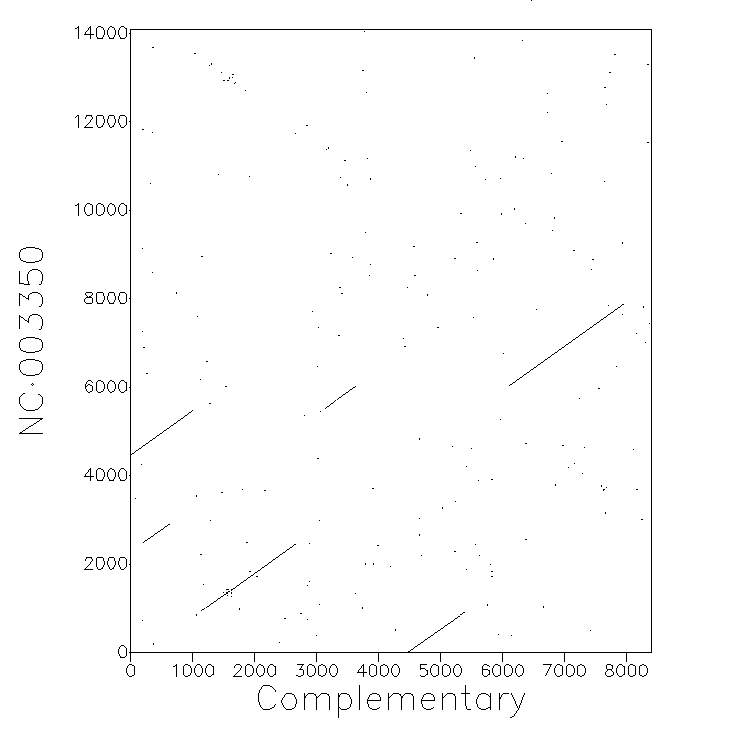
\includegraphics[scale= 0.7]{../res/cible4-ic.png}
			 Séquence complémentée et inversée
		\end{center}
	\end{minipage}
	\caption{Résultat de la collection 4}
	\label{cible4}
\end{figure}

\FloatBarrier

\subsubsection*{Cible 5}


Pour la dernière cible (voir figure~\ref{cible5}), nous obtenons aussi plusieurs segments de droites,
plus ou moins grands, recouvrant la majorité de la séquence cible (un peu plus
de 90\%). Les endroits où les deux séquences ne correspondent pas se situent aux
alentours de 3000 et 7500. Le complémentaire inversé remplit également une bonne
partie de la séquence cible mais il y a plus d'intervalles où les séquences ne
correspondent pas.

Comme pour les séquences précédentes, notre algorithme nous renvoie une séquence
plus longue (environ 6000 nucléotides de plus).

\begin{figure}[!ht]
	\begin{minipage}[r]{.46\linewidth}
		\begin{center}
		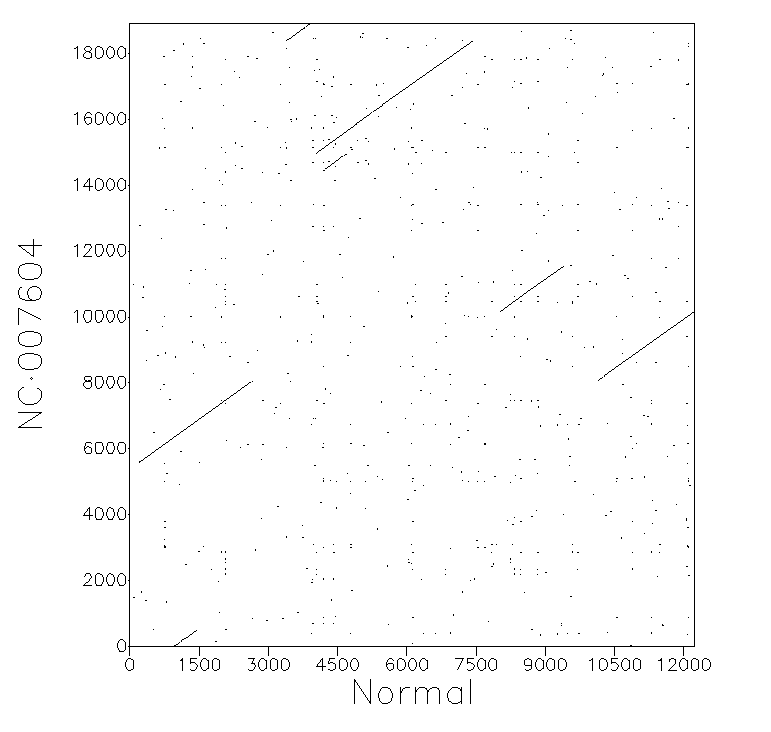
\includegraphics[scale= 0.7]{../res/cible5.png}
Séquence obtenue	\end{center}
\end{minipage} \hfill
\begin{minipage}[c]{.46 \linewidth}
	\begin{center}
			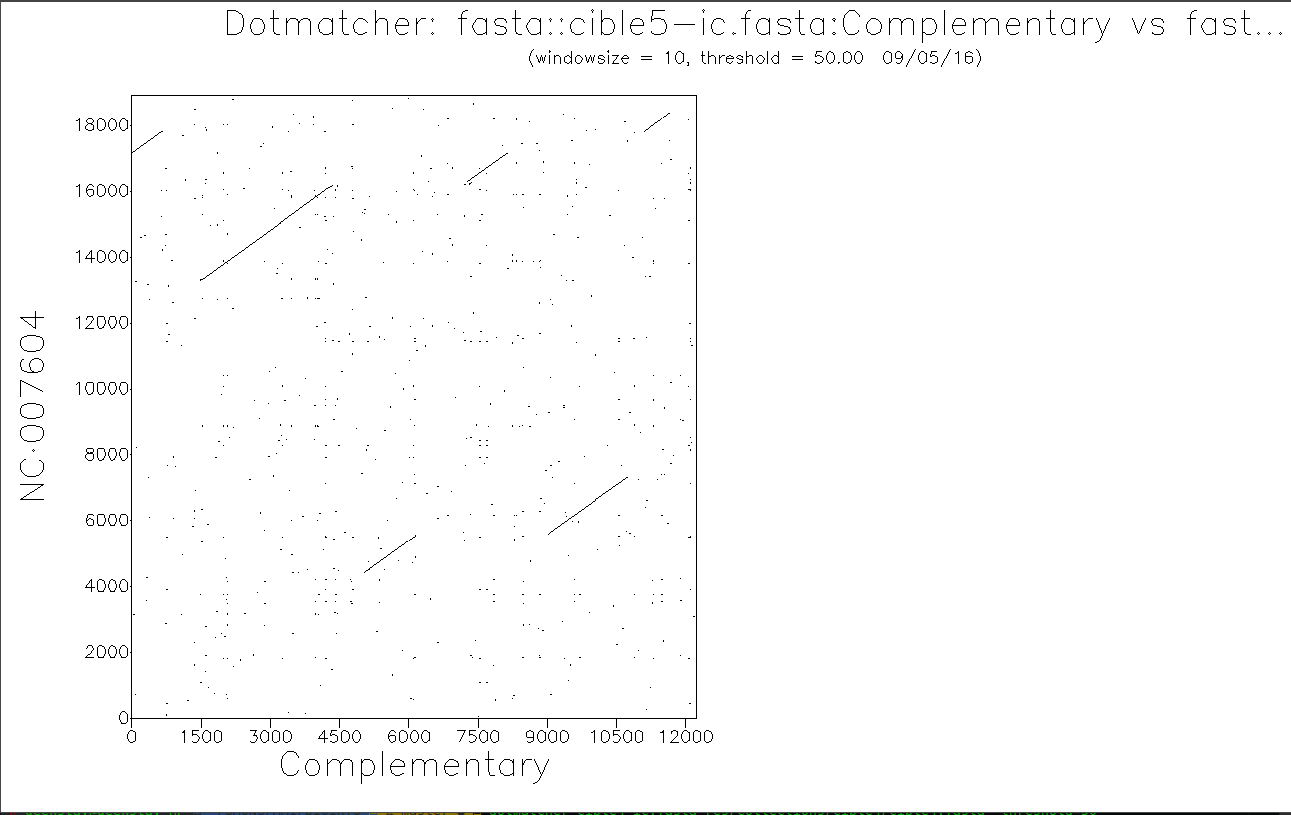
\includegraphics[scale= 0.7]{../res/cible5-ic.png}
			 Séquence complémentée et inversée
		\end{center}
	\end{minipage}
	\caption{Résultat de la collection 5}
	\label{cible5}
\end{figure}

\FloatBarrier


\subsubsection*{Interprétation générale}

De manière générale, nous recouvrons globalement chaque séquence, (jusqu'à 90\%
pour la cible 4), soit de manière continue (longue droite, comme les cibles 1 et
4), soit un peu éparpillé (segments de droite recouvrant de 10 à 40\%, cible 5),
soit très peu de segments et très éparpillé (très petits segments de droites lors
du zoom, cible 2).

Chaque séquence obtenue est plus grande que la séquence cible.

\subsection{Autres implémentations}

Nous avons également expérimenté le changement de \og comportement \fg~de l'algorithme glouton en modifiant
le comparateur d'arcs pour privilégier les alignements ayant une plus grande
sous-séquence commune.

Lorsque deux arcs ont un même score d'alignement, nous avons pour cela
privilégié les arcs qui ont une plus longue sous-séquence commune. Cette méthode
nous a donné des résultats équivalents si ce n'est que les droites apparaissent
plus bas sur le graphe. Sur la figure \ref{fig:autre_impl_4} est représentée le
dotmatcher obtenu sur la collection 4 avec ce nouveau comparateur d'arc. Les
autres dotmatchers donnent la même chose si ce n'est que la projection des segments sur l'axe Y n'est pas au même endroit.

\begin{figure}[!ht]
	\begin{minipage}[r]{.46\linewidth}
		\begin{center}
			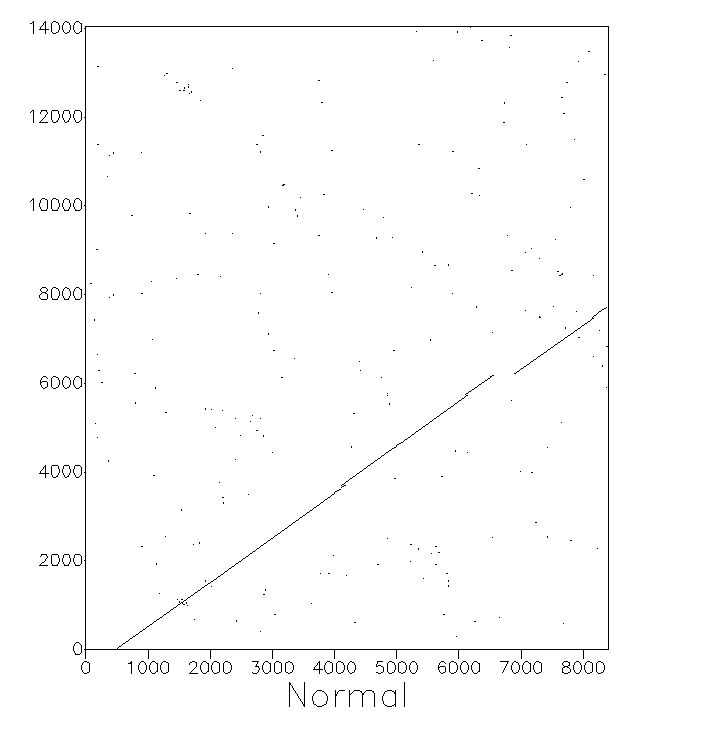
\includegraphics[scale= 0.4]{../res/cible4-other.png}
			Autre implémentation: collection 4
		\end{center}
	\end{minipage} \hfill
	\begin{minipage}[c]{.46\linewidth}
		\begin{center}
		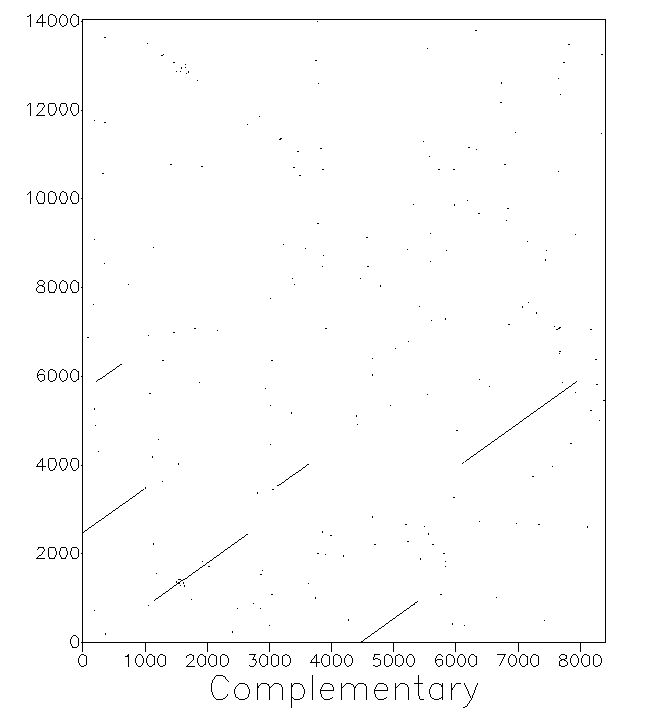
\includegraphics[scale= 0.4]{../res/cible4-ic-other.png}
		Autre implémentation: collection 4, complémenté et inversé
	\end{center}
	\end{minipage}
	\label{fig:autre_impl_4}
	\caption{Autre implémentation: collection 4}
\end{figure}

\FloatBarrier

Dans le code soumis, nous avons prévilégié, lors de l'alignement semi-global,
l'alignement avec le moins de gaps finaux et initiaux, c'est-à-dire en
prenant le dernier maximum pour la dernière colonne et la dernière ligne. Nous
avons tenté de prendre le premier maximum pour chacun d'entre eux, mais cela n'a
pas donné de meilleurs résultats.

%Explication de la propagations des gaps à la fin.

%!TEX root=rapport.tex

\section{Forces et faiblesses de notre travail}

\subsection{Forces}

Le multi-threading de la génération des arcs ainsi que lors du recalcul des alignements associés aux arcs choisis pour le chemin hamiltonien, nous a permis d'améliorer sensiblement la vitesse d'exécution de notre algorithme glouton. A titre d'exemple, nous sommes passés de $\approx 50$ secondes à $\approx 25$ secondes pour le calcul des arcs de la première collection sur la machine d'Aline (MacBook Pro, 2,8 GHz Intel Core i5). Nous avons donc bon espoir quant au fait que, sur des machines pouvant supporter plus de threads, la diminution du temps d'exécution reste proportionnelle à l'augmentation du nombre de threads. De ce fait, nous pouvons récupérer les résultats de la reconstruction de la séquence initiale pour les différentes collections en un temps raisonnable. La collection 2, la plus coûteuse en temps, prend environ une heure de calcul.\\

Nous pensons que l'implémentation de la structure de données Union-Find est particulièrement adaptée dans le cadre de l'implémentation de l'algorithme glouton. La complexité amortie pour les opérations sur cette structure étant en temps constant, il semble difficile de faire mieux.\\

L'implémentation de tests unitaires nous a permis de valider indépendamment chaque partie de notre implémentation.\\

Les méthodes utilisées sont génériques, elles s'appliquent aussi pour n'importe quelles séquences linéaires avec recouvrement partiel (en particulier pour de l'ARN). Au point de vue du code, il n'est nécessaire que de modifier quelques valeurs dans la classe \verb|Nucleotide|.\\

La seconde implémentation des séquences utilisées pour la propagation des gaps
fournit des algorithmes quadratiques en la taille de la plus grande séquence initiale et
du nombre de séquences ainsi qu'un code clair et court. De plus, cette
implémentation peut être généralisée à une liste quelconque d'acides aminés.


\subsection{Faiblesses}

Bien que nous ayons réfléchi à la question, un traitement efficace des alignements de type \og inside\fg~n'a pu être mis en place. Toutefois, l'information nécessaire pour le traitement des arcs représentant des alignements de ce type a été mis en place et une amélioration future peut être effectuée sans devoir changer la structure des objets utilisés pour l'exécution de l'algorithme glouton.\\

Chaque nucléotide est représenté par un byte (8 bits). Or, nous travaillons sur un alphabet de 5 lettres (3 bits nécessaires). Il y aurait donc moyen de faire mieux, mais Java n'est pas très adapté. Nous avons donc dû trouver un compromis entre le temps de calcul et l'allocation mémoire nécessaire.\\

De plus, le passage des objets de classe \verb|Sequence| aux objets de la classe
\verb|SequenceAbstract| prend un temps de calcul $O(M_{i} * k)$, où $M_{i}$ est
la taille de la plus grande séquence initiale et $k$ le nombre initial de
séquences.\\

Bien que l'insertion de gaps lors de la propagation soit
linéaire en la taille de la séquence initiale, ceci étant du à la nécessité de
récupérer la position absolue, il aurait été intéressant d'avoir une complexité
en $O(1)$. Cependant, nous n'avons pu trouver de solutions pour amortir cette
complexité. Le temps constante aurait permis d'arriver à une complexité globale
(pour l'alignement et le consensus) en $O(M_{i} k ^{2})$ à la place de
$O(M_{i}^{2} k^{2})$.\\

Les résultats que nous obtenons pour la cible 2, très différents des autres qui
sont pourtant positifs, sont remplis de bruit avec peu de segments de droite.

%!TEX root=rapport.tex
\section{Organisation du travail}

Lors de la réalisation de ce travail, les tâches réalisées par chacun sont les suivantes:\\
Aline a :
\begin{itemize}
	\item[$\bullet$]Implémenté la lecture et l'écriture de fichiers fasta;
	\item[$\bullet$]Implémenté l'algorithme d'alignement semi-global;
	\item[$\bullet$]Réfléchi quant à la meilleure manière de représenter les ensembles liés à chaque fragment pour l'algorithme Greedy.
	 Cette réflexion a mené à l'implémentation de la structure de données \verb|Union-Find|;
	\item[$\bullet$]Implémenté l'algorithme Greedy et multi-threadé le calcul d'arcs nécéssaires pour la réalisation de l'algorithme Greedy, une fois que celui-ci semblait suffisamment stable.
\end{itemize}
$ $\\
Danny a:
\begin{itemize}
	\item[$\bullet$] Implémenté l'alignement des séquences à partir du chemin hamiltonien;
	\item[$\bullet$] Implémenté le consensus final;
	\item[$\bullet$] % parsing de la command line et du build xml pour le jar.
	\item[$\bullet$] Implémenté la classe \verb|SequenceAbstract| pour
		représenter de manière différente les séquences pour l'alignement
		(voir \ref{subsubsection:repr_sequence_alignment}).
\end{itemize}

Nous avons également eu une discussion préalable afin de réfléchir quant au meilleur moyen de stocker une séquence d'ADN, plus tard Aline a spécifié par quel type d'objet serait représenté le chemin hamiltonien permettant de retrouver la séquence finale et enfin nous nous sommes interrogés ensemble quant à notre compréhension commune de la propagation des gaps pour l'alignement des séquences.
\begin{comment}
De plus, Aline ayant également réfléchi à la manière d'obtenir la séquence finale à partir du chemin hamiltonien donné par l'algorithme greedy avant que Danny ne propose sa propre solution, elle a également exposé son point de vue quant à la réalisation de cette dernière étape. Le temps lui ayant manqué, son algorithme n'est pas totalement abouti et nous avons donc continué de travailler à partir de celui de Danny.
\end{comment}

Enfin, quant à la réalisation de ce rapport, nous l'avons réalisé à deux, chacun se concentrant surtout sur l'explication des parties du travail qu'il a réalisé.

%!TEX root=rapport.tex

\section{Conclusion}
\end{document}
